\documentclass[UTF8]{ctexart}
\usepackage{graphicx}
\usepackage{multirow}
\usepackage{booktabs}
\usepackage{latexsym}
\usepackage{indentfirst}
\setlength{\parindent}{2em}
\usepackage{color}
\definecolor{lbcolor}{rgb}{0.9,0.9,0.9}
\usepackage{listings}
\lstset{backgroundcolor=\color{lbcolor}}
\lstset{keywordstyle=\color[rgb]{0,0,1}}
\lstset{commentstyle=\color[rgb]{0.133,0.545,0.133}}
\lstset{stringstyle=\color[rgb]{0.627,0.126,0.941}}
\lstset{language=Matlab}
\lstset{numbers=left}
\lstset{breaklines=true}
\author{何舜成}
\date{2012011515}
\title{Image Processing Exercise 3}
\begin{document}
\maketitle
\section{问题描述}
下图是某生产厂商的传送带成像图,用适当的方法\par
(1)找出图中有几个瓶子;\par
(2)检测出未装满的瓶子。\par
\begin{figure}[htbp]
\centerline{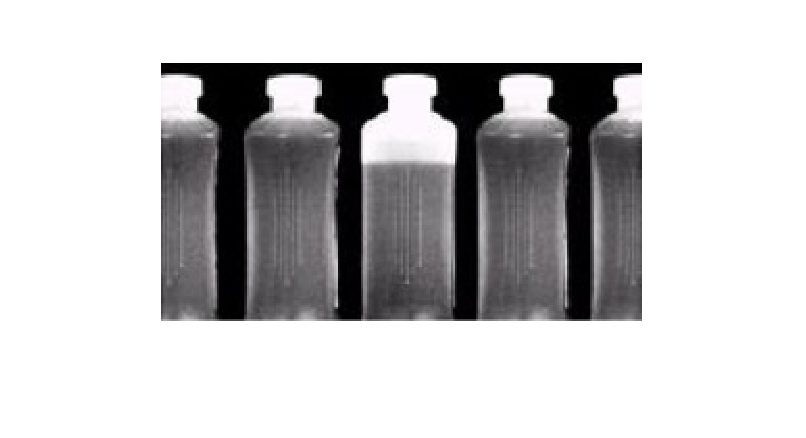
\includegraphics[width=3.5in]{origin.eps}}
\caption[]{original image}
\end{figure}
\section{问题解答}
明显可以看到,瓶子和背景之间灰度值有明显差异,而瓶子空的部分与瓶子本身之间也有灰度值差异,因此可以根据阈值二值化来分割出瓶子空的部分,如图2\par
\begin{figure}[htbp]
\centerline{
\includegraphics[width=3.5in]{thres.eps}}
\caption[]{binary image w.r.t. threshold}
\end{figure}\par
由于噪声的存在,我们必须对背景做一次膨胀操作,使得前景连通区域个数等于瓶子的个数,膨胀过后如图3\par
\begin{figure}[htbp]
\centerline{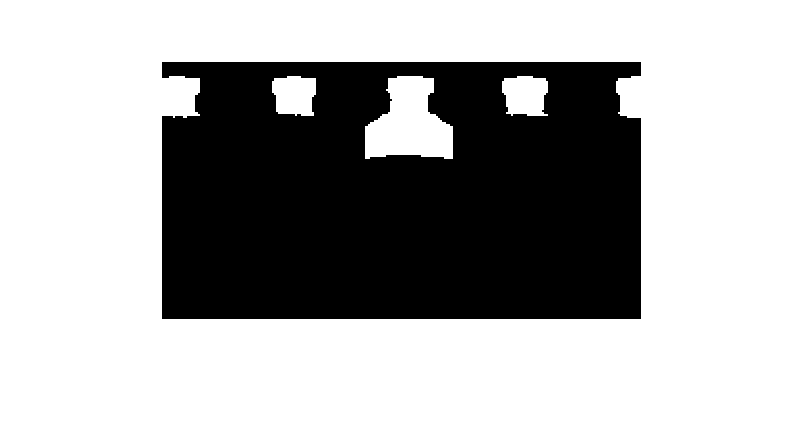
\includegraphics[width=3.5in]{diluted.eps}}
\caption[]{background diluted}
\end{figure}\par
下面是连通区域计数的方法,我们可以先对行进行间隔编码,然后遍历所有行给不同连通区域编号,在实际操作中,两个步骤合到一起了。图4的不同灰度值代表了不同的连通区域。\par
\begin{figure}[htbp]
\centerline{
\includegraphics[width=3.5in]{class.eps}}
\caption[]{connected areas}
\end{figure}\par
根据连通区域面积大小可以知道,面积显著偏大的那一块面积对应的是未装满的瓶子,如图5标红的区域。\par
\begin{figure}[htbp]
\centerline{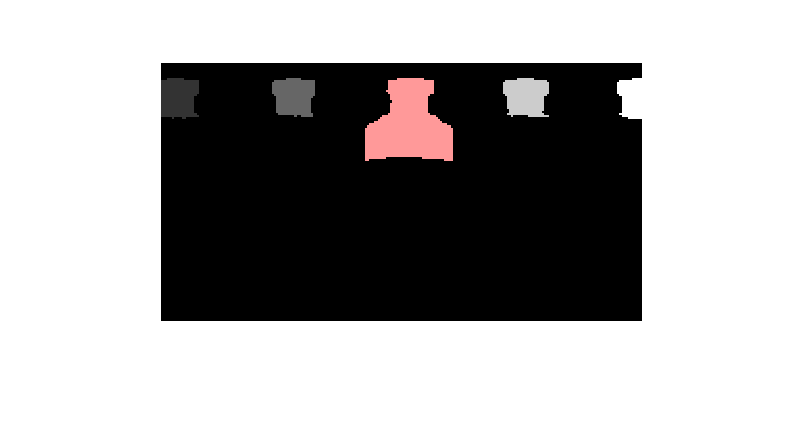
\includegraphics[width=3.5in]{empty.eps}}
\caption[]{unfilled bottle}
\end{figure}\par
源码为Matlab,运行环境为Matlab R2013a,Mac OS X版。
\end{document}